\documentclass[12pt,letterpaper]{article}
% The usepackage tell LaTeX which packages are needed. As you get better you can add more
% packages for extra functionality
% Percent signs are comments, they will not be read by the renderer.
\usepackage{fullpage}
\usepackage[top=2cm, bottom=2.5cm, left=2.5cm, right=2.5cm]{geometry}
\usepackage{amsmath,amsthm,amsfonts,amssymb,amscd}
\usepackage{lastpage}
\usepackage{enumerate}
\usepackage{fancyhdr}
\usepackage{mathrsfs}
\usepackage{xcolor}
\usepackage{graphicx}
\usepackage{multicol}
\usepackage{wrapfig}
\usepackage{hyperref}
\usepackage{systeme}
\usepackage{subfig}
\usepackage[shortlabels]{enumitem}
\usepackage{listings} %for listings of the source code
\usepackage{tikz}
\usetikzlibrary{shapes,arrows,chains}

% Some definitions for using the listing package.
% When we reference 'codegreen', it will be the RGB color defined below.
\definecolor{codegreen}{rgb}{0,0.6,0}
\definecolor{codegray}{rgb}{0.5,0.5,0.5}
\definecolor{codepurple}{rgb}{0.58,0,0.82}
\definecolor{backcolour}{rgb}{0.95,0.95,0.92}
\DeclareUnicodeCharacter{2212}{-}

% Also for the listings, this will make the code listing look like default MATLAB
\lstdefinestyle{mystyle}{
	backgroundcolor=\color{backcolour},   
	commentstyle=\color{codegreen},
	keywordstyle=\color{magenta},
	numberstyle=\tiny\color{codegray},
	stringstyle=\color{codepurple},
	basicstyle=\footnotesize,
	breakatwhitespace=false,         
	breaklines=true,                 
	captionpos=b,                    
	keepspaces=true,                 
	numbers=left,                    
	numbersep=5pt,                  
	showspaces=false,                
	showstringspaces=false,
	showtabs=false,                  
	tabsize=2
}
\lstset{style=mystyle}

\hypersetup{%
  colorlinks=true,
  linkcolor=blue,
  linkbordercolor={0 0 1}
}
 
\setlength{\parindent}{0.0in}
\setlength{\parskip}{0.05in}

\newcommand\course{COMP 521}
\newcommand\hwnumber{8}             
\newcommand\MyName{Zack Humphries}  

\pagestyle{fancyplain}
\headheight 15pt
\lhead{\MyName}
%\lhead{\NetIDa\\\NetIDb}                 % <-- Comment this line out for problem sets (make sure you are person #1)
\chead{\textbf{\Large Homework \hwnumber}}
\rhead{\course\\ December 9, 2022}
\lfoot{}
\cfoot{}
\rfoot{\small\thepage}
\headsep 1.5em

\begin{document}

\section*{Problem 1}
The graph in figure \ref{fig001} shows the connection between four different web pages a, b, c and d. Rank the web pages using the approach based on the Perron-Frobenius eigenvector. Show the matrices used to solve the problem.

\begin{figure}[h]
	\centering
	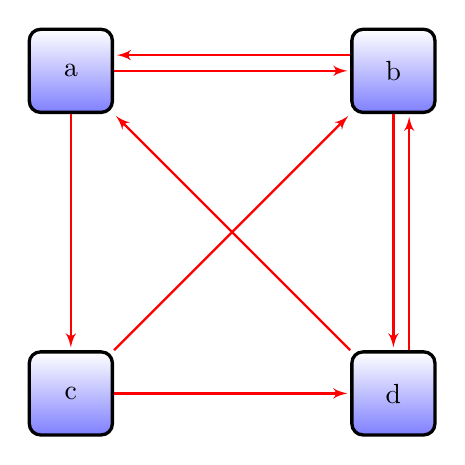
\begin{tikzpicture}[node distance=1cm, auto]  
	\tikzset{
		mynode/.style={rectangle,rounded corners,draw=black, top color=white, bottom color=blue!50,very thick, inner sep=1em, minimum size=3em, text centered},
		myarrow/.style={red,->, >=latex', shorten >=1pt, thick},
		mylabel/.style={text width=7em, text centered} 
	}  
	\node[mynode] (a) {a};  
	\node[mynode, right=3cm of a] (b) {b}; 
	\node[mynode, below=3cm of a] (c) {c};  
	\node[mynode, below=3cm of b] (d) {d};
	
	\draw[myarrow] (a.south) --  (c.north);	
	\draw[myarrow] (a.east) --  (b.west);
	
	\draw[myarrow] ([shift={(0mm,2mm)}] b.west) -- ([shift={(0mm,2mm)}] a.east);	\draw[myarrow] (b.south) -- (d.north);
	
	\draw[myarrow] (c.east) -- (d.west);
	\draw[myarrow] (c) -- (b);
	
	\draw[myarrow] (d) -- (a);
	\draw[myarrow] ([shift={(2mm,0mm)}] d.north) -- ([shift={(2mm,0mm)}] b.south);
	
	\end{tikzpicture}
	\caption{Links between four web pages}  \label{fig001}
\end{figure}

The adjacency matrix from the figure above is\ldots
\begin{equation*}
    A =
    \begin{bmatrix}
        0 & \frac{1}{2} & 0 & \frac{1}{2} \\ \frac{1}{2} & 0 & \frac{1}{2} & 0 \\ \frac{1}{2} & 0 & 0 & 0 \\ 0 & \frac{1}{2} & \frac{1}{2} & 0
    \end{bmatrix}
\end{equation*}

The page rank $\overrightarrow{x}$ is calculated by using M

\begin{equation*}
    M = dA + \frac{(1-d)}{4}
    \begin{bmatrix}
        1 & 1 & 1 & 1 \\ 1 & 1 & 1 & 1 \\ 1 & 1 & 1 & 1 \\ 1 & 1 & 1 & 1
    \end{bmatrix}
\end{equation*}


Where $d=0.85$. The resulting $\overrightarrow{x}$ is recalculated by being multiplied by $M$ over and over again until the difference in the vector L2-norm is less than $10^{-6}$ or the iterative process has run more than $10000$ times.
Displayed in the code below\ldots


\lstset{title={Problem 1 Iterative Process}}
\begin{lstlisting}[language = Matlab]
x = ones(n, 1);
diff = x;
count = 1; maxiter = 10000;

while norm(diff) > 1e-6 && count < maxiter
    xold = x;
    xnew = M * x;
    diff = xnew - xold;
    x = xnew;
    count = count + 1;
end
\end{lstlisting}

After the iterative process is done, $\overrightarrow{x}$ is divided by its resulting L2-norm, providing the answer\ldots

\begin{equation*}
    \overrightarrow{x} =
    \begin{bmatrix}
        0.5777 \\ 0.0298 \\ 0.3587 \\ 0.5069
    \end{bmatrix}
\end{equation*}

This answer can be compared to the first column vector (which corresponds to the highest postivive eigenvalue from $\Lambda$, $0.8908$, satisfying the Perron-Frobenius Theorem) from the resulting $V$ from Singular Value Decomposition\ldots

\begin{equation*}
    V_{1} =
    \begin{bmatrix}
        0.5777 + 0.0000i \\ 0.5298 + 0.0000i \\ 0.3587 + 0.0000i \\ 0.5069 + 0.0000i
    \end{bmatrix}
\end{equation*}

$V_1$ reaffirms $\overrightarrow{x}$ from the iterative process is correct, showing that rank from most to least important webpage would be in the order of $a$, $d$, $c$, and finally $b$.



\newpage
\section*{Problem 2}
Choose an image of your preference and analyze it using PCA. Describe your work step by step and show figures/plots to support your results. You can do either an RGB or greyscale image.

I chose the following greyscaled image of my boyfriend and me on his grandparent's farm:

\begin{figure}[!h]
    \centering
    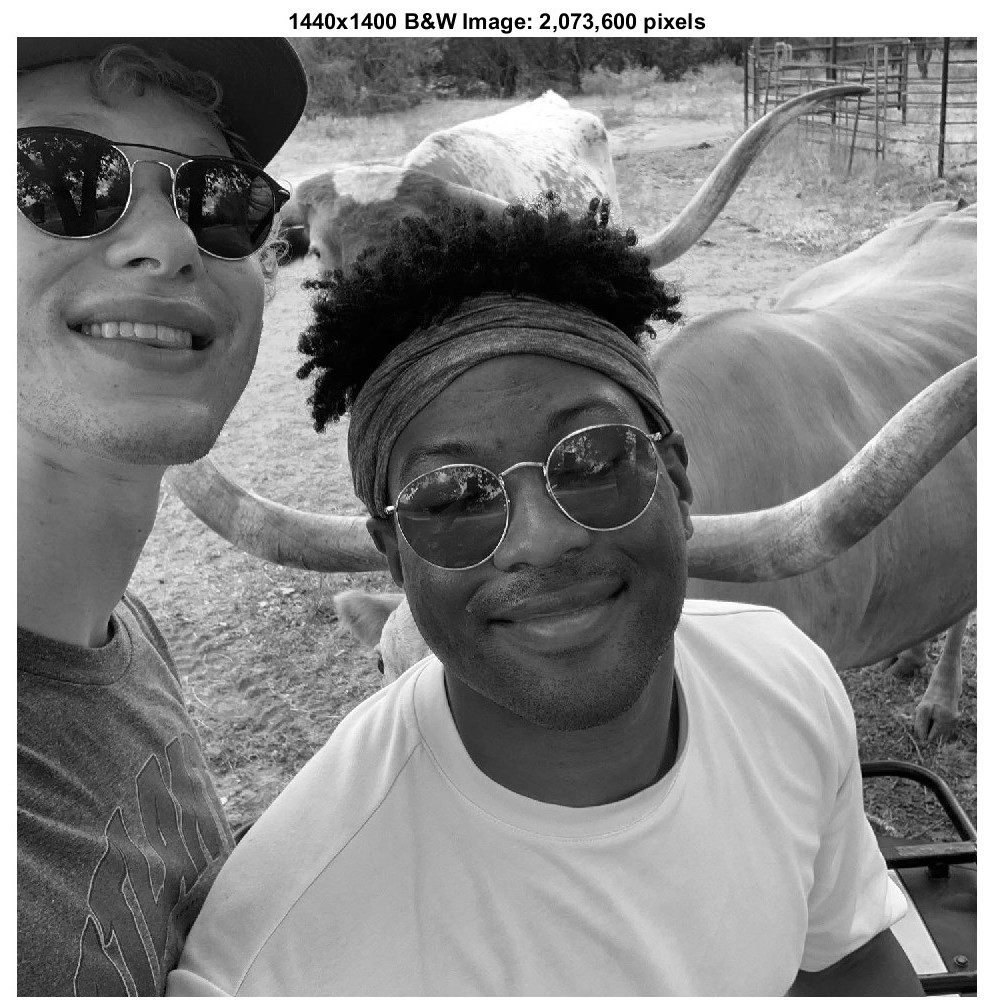
\includegraphics[width = 1\textwidth]{Z_Z_BW.jpg}
    \caption{Problem 2: Original Picture}
\end{figure}

I felt that there was a lot of complexity to this image and wanted to see how many principal components would need to be used to recreate the image without any noticable changes.

After some tinkering with the principal components array, I found that 300 principal components created no noticible changes, which will be shown and discussed later.

\subsection*{Step-By-Step Process Applied to the Image}

The following steps describe the process applied the the image in order to find the principal components and recreate an indistinguishable image with only 300 principal components\ldots


\begin{enumerate}
    \item Read the image and convert the image to grey values
    
    The image is read by the function, \emph{imread}, and converted to grayscale values (ranging from 0 to 255) by the function, \emph{rgb2gray}. The process is displayed by the following code\ldots
\lstset{title={Read and Convert to Grayscale Values}}
\begin{lstlisting}[language = Matlab]
% Read in image
I = imread('Z_Z.jpg'); 
% and convert to grayscale
I = rgb2gray(I);
\end{lstlisting}

    \item Center the data
    
    The greyscale matrix is subtracted by the mean of the values in each column of the matrix\ldots
\lstset{title={Centering the Data}}
\begin{lstlisting}[language = Matlab]
% Make data double precision
data = double(I);
%
[m n] = size(data);

% Find mean
mn   = mean(data,1);

% make data have zero mean, for covariance
data = data - repmat(mn,m,1);
\end{lstlisting}

    \item Compute the covariance matrix
    
    This process is done by the function, \emph{cov}
\lstset{title={Computing Covariance Matrix}}
\begin{lstlisting}[language = Matlab]
% Find covariance of the data
covar_temp = cov(data);
\end{lstlisting}

    \item Find the eigenvectors and eigenvalues of the covariance matrix
    
    This process is done by the function, \emph{eig}, which is then flipped to have the eigenvectors/values go from largest to smallest
\lstset{title={Finding Eigenvectors/values of the Covariance Matrix}}
\begin{lstlisting}[language = Matlab]
% Find eigen values and vectors, returns eigenvalues as vector
[PC, V] = eig(covar_temp, 'vector');

% Flip values and vectors to go from biggest to smallest
V  = flipud(V);
PC = fliplr(PC);
\end{lstlisting}

    \item Reconstruct the image using different numbers of principal components
    
    For this analysis, I chose six principal component thresholds: $[1, 10, 50, 100, 200, 300]$

    The process for recreating the image by multiplying the principal component matrix with the number of principal component vectors equal to that of the principal component threshold with the average being added back to it and then readjusted is shown below\ldots

\lstset{title={Reconstructing the Image}}
\begin{lstlisting}[language = Matlab]
% Loop over different PC sizes and plot them
pc = principal_components; 
figure(34); 
vsum = sum(V);
tiledlayout(3,2)
for pp = 1:pics
    % Extract the principal components we asked for
    output = PC(:,1:(pc(pp)))' * data';
    [xx yy] = size(output); ts = (xx+1)*yy;
    % Reconstruct full image from those principal components ( round for
    % greyscale values, need to be whole numbers )
    reconstruct = round((PC(:,1:(pc(pp)))*output) + repmat(mn,m,1)');

    % Show reconstructed image with n principal components
    nexttile
    imshow(reconstruct', []);
    title([num2str(pc(pp)) ' components, ' num2str((ts)/(m*n)*100) '%  storage, ' num2str(sum(V(1:pc(pp))/vsum)*100) '% eigen']);
end

figure(99)
    imshow(reconstruct', []);
    title([num2str(pc(pp)) ' components, ' num2str((ts)/(m*n)*100) '%  storage, ' num2str(sum(V(1:pc(pp))/vsum)*100) '% eigen']);
\end{lstlisting}   

\newpage
    The resulting images show a gradual increase in clarity. Using only 200 principal components was nearly indistinguishable from the original image, however, the next 100 principal components struggled to accurately depict the stubble on our faces.

\begin{figure}[!h]
    \centering
    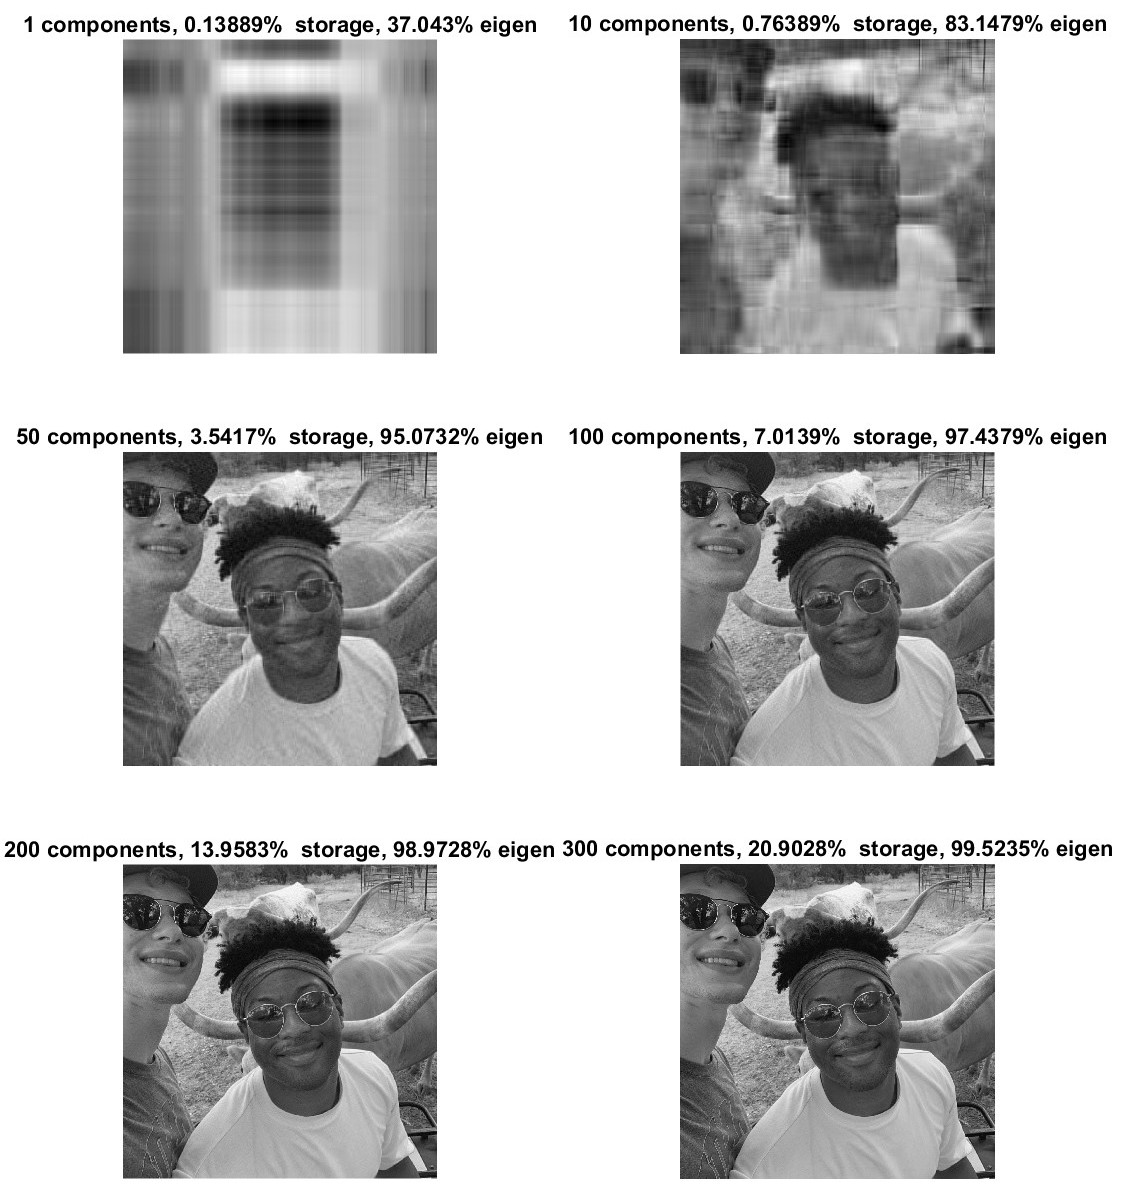
\includegraphics[width = 1\textwidth]{Z_Z_diff_3_2.jpg}
    \caption{Problem 2: Pictures from PCA Analysis}
\end{figure}

\end{enumerate}

\newpage
The final image uses only $300$ of the $1440$ principal components, however, those factors for more than $99.5\%$ of the sum of all of the eigenvalues.

\begin{figure}[!h]
    \centering
    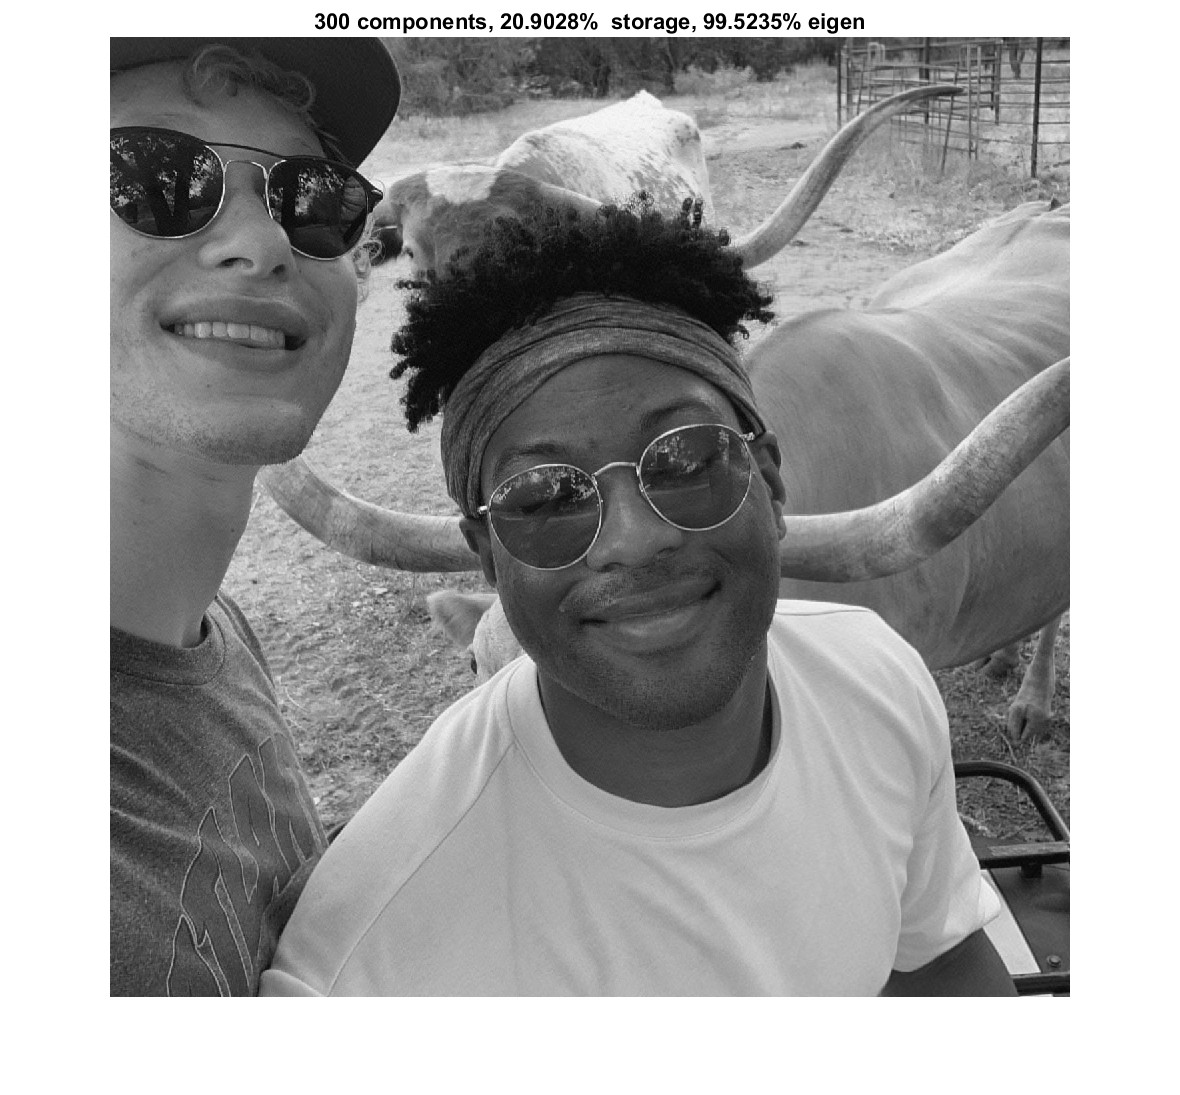
\includegraphics[width = 1\textwidth]{Z_Z_BW_300.jpg}
    \caption{Problem 2: Resulting Image Using Only 300 Principal Components}
\end{figure}

\newpage
\section*{MATLAB Code}
\lstset{title={Problem 1}}
\begin{lstlisting}[language = Matlab]
%% Adjacency Solver

close all; clear all; clc;

A = [ 0    1/2   0  1/2; ...
      1/2   0   1/2  0; ...
      1/2   0    0   0; ...
      0    1/2  1/2  0];

d = 0.85;

[m n] = size(A);


M = d .* A + ((1-d)/n)*ones(size(A));

x = ones(n, 1);
diff = x;
count = 1; maxiter = 10000;

while norm(diff) > 1e-6 && count < maxiter
    xold = x;
    xnew = M * x;
    diff = xnew - xold;
    x = xnew;
    count = count + 1;
end
x_norm = x / norm(x);

disp(x_norm)

% Check with eigen values / vectors
[V L] = eig(M);

% Largest eigen value
L

% matches eigen vector (+/- sign)
V
\end{lstlisting}

\lstset{title={Problem 2}}
\begin{lstlisting}[language = Matlab]
%% Greyscale PCA
%
% Jared Brzenski

close all;
clear all;
clc
% Setup principal components to use. Pick 4.
principal_components = [1 10 50 100 200 300]
pics = length(principal_components);

% Read in image
I = imread('Z_Z.jpg'); 
% and convert to grayscale
I = rgb2gray(I);

% Show it
figure(1)
imshow(I, []);title('1440x1400 B&W Image: 2,073,600 pixels'); 

% Make data double precision
data = double(I);
%
[m n] = size(data);

% Find mean
mn   = mean(data,1);

% make data have zero mean, for covariance
data = data - repmat(mn,m,1);
fprintf('Now data has zero mean: %4.5f\n', (mean(mean(data))) );

% Find covariance of the data
covar_temp = cov(data);
%
% Or do it by hand....
% for y=1:n
%     for in=1:n
%             covar_temp(y,in)=1/((m*n)-1)*(data(:,y)' * data(:,in))  ;
%     end
% end
%
% Find eigen values and vectors, returns eigenvalues as vector
[PC, V] = eig(covar_temp, 'vector');

% Flip values and vectors to go from biggest to smallest
V  = flipud(V);
PC = fliplr(PC);

% OLD!!!: Rank and order the values and vectors
%%%%%%%%%%%%%%%%%%%%%%%%%%%%%%%%%%%%%%%%%%%%%%%%%%%%%%%%%%%%%
% Retain only the eigen values ( stored on the diagonal )
%V = diag(V);

% Rank the eigenvalues - backwards from given values
%[holder rank_indices] = sort(-1*V);

% Sort the eigen vectors based on the sorted eigenvalues
%V = V(rank_indices);
%PC = PC(:,rank_indices);
%%%%%%%%%%%%%%%%%%%%%%%%%%%%%%%%%%%%%%%%%%%%%%%%%%%%%%%%%%%%

% Loop over different PC sizes and plot them
pc = principal_components; 
figure(34); 
vsum = sum(V);
tiledlayout(3,2)
for pp = 1:pics
    % Extract the principal components we asked for
    output = PC(:,1:(pc(pp)))' * data';
    [xx yy] = size(output); ts = (xx+1)*yy;
    % Reconstruct full image from those principal components ( round for
    % greyscale values, need to be whole numbers )
    reconstruct = round((PC(:,1:(pc(pp)))*output) + repmat(mn,m,1)');

    % Show reconstructed image with n principal components
    nexttile
    imshow(reconstruct', []);
    title([num2str(pc(pp)) ' components, ' num2str((ts)/(m*n)*100) '%  storage, ' num2str(sum(V(1:pc(pp))/vsum)*100) '% eigen']);
end

figure(99)
    imshow(reconstruct', []);
    title([num2str(pc(pp)) ' components, ' num2str((ts)/(m*n)*100) '%  storage, ' num2str(sum(V(1:pc(pp))/vsum)*100) '% eigen']);
\end{lstlisting}

\end{document}